\documentclass[output=paper]{langsci/langscibook}
\ChapterDOI{10.5281/zenodo.3972864}

\author{Xuhui Hu\affiliation{Peking University}}

\title[Functional items, lexical information, and telicity]
      {Functional items, lexical information, and telicity:\newlineCover{} A parameter hierarchy-based approach to the telicity parameter}
      [Functional items, lexical information, and telicity: A parameter hierarchy-based approach to the telicity parameter]

\abstract{This paper attempts to present an account for the \isi{parameters} of
    telicity based on data from \ili{Yixing Chinese}, a variety of Chinese Wu
    dialect, as well as well-studied languages like \ili{English} and Slavic
    languages. It is argued that the cross-linguistic variation of telicity is
    reduced to two factors of a lexicon: whether a language has a functional
    item bearing a telic (quantity) feature, and whether the telic functional
    item also bears extra semantic information entailing the measuring up point
    of the event. These two factors determine the following properties of a
    language: in \ili{English} and other \ili{Germanic} languages, without a telic
    functional item, telicity often relies on quantity objects, and a quantity
    object often forces telic interpretation to be derived; in \ili{Slavic} languages
    and Chinese (Mandarin, Yixing and perhaps other dialects) wherein telic
    \isi{functional items} are available, telicity does not rely on quantity objects
    but on the functional item, which imposes quantification over bare
    nominals. \ili{Slavic} languages differ from Chinese in that their telic items
    also bear semantic information entailing the measuring up point of an
    event, so the endpoint of a telic event is invariably identified with its
    measuring up point, while such information is only a piece of cancellable
    default meaning in Chinese.}
\maketitle

\begin{document}\glsresetall

\section{Introduction}\label{sec:17.1}

This paper studies the syntactic variation of \isi{inner aspect}, which is
concerned with the internal temporal structure of an event, as opposed to outer
aspect \citep[7]{travis1991} that denotes the speaker's point of view over the
event \citep{smith1997parameter}. While outer aspect is uniformly taken as a
syntactic object realised by a functional head\is{functional items} (Asp head) in the syntactic tree
of the Chomskyan tradition, ever since \citeauthor{vendler1957verbs}'s
(\citeyear{vendler1957verbs}) work, \isi{inner aspect} has been widely taken as
part of lexical information, characterised by the classification of the
accomplishment, achievement, activity, and state predicates. However, recently,
researchers like \textcite{Borer2005a,Borer2005b,Borer2013},
\textcite{MacDonald2008} and \textcite{travis2010inner} come to the conclusion
that \isi{inner aspect}, like outer aspect, is also an interpretation derived
from syntactic computation, instead of being a piece of lexical information. In
this paper, drawing on new data from a Chinese dialect, Yixing, I take up this
assumption, especially that of \textcite{Borer2005a,Borer2005b,Borer2013}, to
further investigate the underlying mechanism leading to the cross-linguistic
variation of \isi{inner aspect}.

Variation concerning \isi{inner aspect}, especially telicity, has been widely
discus\-sed in \textcite{filip1997,filip2000}, \textcite{filiprothstein2005},
\textcite{Borer2005a,Borer2005b}, \textcite{MacDonald2008}, and
\textcite{travis2010inner},  among many others. This paper, drawing upon data
from \ili{Yixing Chinese} described in \textcite{Huxuhui2016}, places Chinese
within the broad picture of comparative study on telicity, and shows that
variation of telicity hinges upon the (un)availability of a functional item
bearing a telic (quantity) feature in the lexicon, and further variation will
arise due to extra semantic flavours of the functional item. This paper,
therefore, not only contributes new data to the debate on the nature of
telicity, but also provides a new account for the variation of telicity in the
manner of hierarchy of \isi{parameters} proposed in \textcite{robertsonline}.

The rest of this paper is organised as follows. \sectref{sec:17.2} presents a sketchy
introduction to telicity related notions and issues in \ili{English} and
\ili{Slavic}
languages that have been covered in the recent study of telicity and its
variation. \sectref{sec:17.3} will present a summary of two approaches to the
cross-linguistic variation of telicity, and \sectref{sec:17.4}, with the presentation of
the data from \ili{Yixing Chinese}, brings Chinese into the picture of the
telicity variation. Based on the data and framework outlined in the previous
sections, in \sectref{sec:17.5} I explain the underlying mechanisms that govern the
variation on telicity, and work out a hierarchy of \isi{parameters} of telicity.
\sectref{sec:17.6} concludes the paper.

\section{Inner aspect and variation: The facts}\label{sec:17.2}

\subsection{Inner aspect: A short introduction}\label{sub:17.2.1}

Inner aspect, also termed as \textit{aktionsart} and \textit{lexical aspect}, is not about how
the language user views an event, but about the internal structure, temporal
structure in particular, of an event. Whether an event is expressed as having
an endpoint is at the centre: an event with an endpoint is assumed to be telic,
otherwise atelic. It should be noted that telicity is not about the reality,
but is a piece of information expressed linguistically:

\begin{exe}
\ex\begin{xlist}
	\ex\label{EnglishTelicitya} John ate an apple in 5 minutes.
    \ex\label{EnglishTelicityb} John ate apples for 10 minutes.
\end{xlist}
\end{exe}

(\ref{EnglishTelicitya}) is telic: the endpoint of the eating event was the
point when the last bit of the apple was consumed. (\ref{EnglishTelicityb}) is
atelic, as the endpoint is not expressed linguistically -- we only know from
the sentence that within 10 minutes, John had been eating apples. While in
reality there will be an endpoint of the event of John's eating apples, this
information is not expressed by the sentence.

If we only take \ili{English} data to explore the nature of \isi{inner aspect}, two factors
are at stake in determining telicity. The first concerns the verb types in
terms of \citeauthor{vendler1957verbs}'s (\citeyear{vendler1957verbs})
classification. Telicity in \ili{English} often goes with achievement and
accomplishment predicates, and it is quite hard to express a telic event if the
predicate is of the activity or state type (but see later that under certain
circumstances, telicity will also arise with such predicates).

\begin{exe}
\ex\begin{xlist}
	\ex\label{VendlerAchievement} John reached the summit at 9 pm.
    \ex\label{VendlerAccomplishment} John drank a bottle of beer in 10 minutes.
    \ex\label{VendlerActivity} John pushed the cart for/*in 10 minutes.
    \ex\label{VendlerState} Mary stayed in London for/*in 10 days.
\end{xlist}
\end{exe}

In the above examples, \emph{reach} is an achievement predicate which denotes a
change of state at a single temporal point -- the initial and the final points
share the same point, i.e. \emph{9 pm} in (\ref{VendlerAchievement}).
\emph{drink} is an accomplishment predicate which in
(\ref{VendlerAccomplishment}) denotes an event that spans a period of time: the
initial point was when John began to drink the beer while the endpoint was when
the final drop of the beer was consumed. In (\ref{VendlerActivity}) and
(\ref{VendlerState}), no endpoint is expressed, which is confirmed by the
incompatibility with the \emph{in x time} adverbial, a standard diagnostic of
telicity. Following \textcite{dowty1991thematic} and
\textcite{Rothstein2004}, the predicates that allow for telicity take
the internal argument as an ``incremental theme'', which is an argument that
seems to measure up the event, representing a homomorphic mapping between the
argument and the event. For example, \emph{a glass of beer} is an incremental
theme in (\ref{VendlerAccomplishment}): there is a one-to-one homomorphic
mapping between the glass of wine and the drinking event: the consumption of
the last drop of the wine signals the endpoint of the drinking event. It is in
this sense that predicates like \emph{drink} are termed as homomorphic
predicates \citep{krifka1992,krifka1998originstelicity,filip1997}, which
include both accomplishment and achievement predicates.

The second factor concerns the internal argument. An accomplishment or
achievement predicate does not guarantee the telicity of an event: often a
quantised or quantity object
\citep{krifka1992,krifka1998originstelicity,Borer2005a,Borer2005b}
is needed. Consider the following examples:

\begin{exe}
\ex\begin{xlist}
	\ex John drank water *in 5 minutes.
    \ex John built houses *in 2 months.
\end{xlist}
\end{exe}

In addition to the aforementioned factors, sometimes a directional PP can also
affect telicity: while an activity predicate normally does not allow for telic
interpretation, the addition of a directional PP can contribute to the telic
interpretation:

\begin{exe}
\ex\begin{xlist}
	\ex John pushed the cart *in 10 minutes.
    \ex John pushed the cart \emph{to the wall} in 10 minutes.
\end{xlist}
\end{exe}

It is clear that it is the PP \emph{to the wall} that makes the telic
interpretation legitimate. Without taking any theoretical stance for now, we
can say that the function of PP is to provide an endpoint to the pushing event.

Relying on \ili{English} data, we can draw a conclusion that telicity connects with
multiple facets: the predicate type (at the level of verbal head, or simply a
matter of lexical information), the quantity of nominal objects (NP or DP
level, definitely not a matter of lexical information), and the function of
the directional PP (VP level). Whatever approach we take, one point is for
sure: telicity is by no means a matter solely confined to the domain of lexical
information.

Another conclusion derived from \ili{English} data is that telicity (or inner aspect)
in \ili{English}, unlike outer aspect, is not represented by morphological marking:
there is no grammatical marker to yield telicity; but outer aspect clearly
represents morphological marking -- the progressive aspect is reflected by the
\emph{ing} marking on the verb, for example.

In the next section, I will show that in some languages, telicity of an event
is not determined equally by the aforementioned factors; moreover, there is
morphological marking directly related to telicity. The existence of such
phenomena makes the variation of telicity an interesting research topic, which
constitutes the central topic of this paper.

\subsection{Telicity in \ili{Slavic} languages}\label{sub:17.2.2}

Slavic languages are often taken as the major source showing the variation of
telicity (but see \citealt{travis2010inner} for more languages). Two points of
Slavic languages are at stake. First, when a telic event is expressed, a
perfective prefix is attached to the verb. The following \ili{Russian} examples
exhibit this point:

\begin{exe}
\ex \ili{Russian} \parencite[146]{MacDonald2008}\begin{xlist}
    \ex \gll Ja vypil butylku vina za čas {/ } \llap{*}{v tečeniji} časa.\\
            I {drank-\Pfv{}} a-bottle of-wine in hour {} during hour \\
	    \glt \enquote*{I drank a bottle of wine in an hour / *for an hour.}
    \ex \gll  Mary pročital knigu za čas {/ } \llap{*}{v tečeniji} časa.\\
            Mary {read-\Pfv{}} a-book in hour {} during hour\\
        \glt \enquote*{Mary read a book/poetry in an hour / *for an hour.}
\end{xlist}
\end{exe}

Recall in \ili{English}, the existence of an accomplishment predicate and a quantity
object can give rise to a telic event; in \ili{Russian}, however, without a
perfective prefix, telicity cannot be yielded:

\begin{exe}
    \ex \ili{Russian} \parencite[146]{MacDonald2008} \begin{xlist}
    \ex \gll Ja pil butylku vina \llap{*}za čas / {v tečeniji} časa.\\
	        I {drank-\Ipfv} a-bottle of-wine in hour {} during hour \\
	    \glt \enquote*{I drank a bottle of wine *in an hour / for an hour.}
    \ex \gll  Mary čitala knigu \llap{*}za čas / {v tečeniji} časa.\\
            Mary {read-\Ipfv} {a book} in hour {} during hour\\
        \glt \enquote*{Mary read a book *in an hour / for an hour.}
\end{xlist}
\end{exe}

While a directional PP can turn an activity event into a telic one, without a
perfective affix, telic interpretation is just impossible in \ili{Russian}:

\begin{exe}
\ex \ili{Russian} \parencite[148]{MacDonald2008} \begin{xlist}
	\ex \gll Fermer tasčil brevno v ambar \llap{*}za čas / {v tečeniji} časa.\\
	        {The farmer} {dragged-\Ipfv} {the log} into {the barn} in hour {} during hour \\
	    \glt \enquote*{The farmer dragged the log into the barn *in an hour / for an hour.}
    \ex \gll  Ptisi leteli k kletke \llap{*}za čas / {v tečeniji} časa.\\
            {The birds} {flew-\Ipfv} toward {their cage} in hour {} during hour\\
        \glt \enquote*{The birds flew toward their cage *in an hour / for an hour.}
\end{xlist}
\end{exe}

While there are more telicity related properties in \ili{Slavic} languages which I
will introduce in the course of discussion, now we can already see some aspects
of variation of telicity: in \ili{Slavic} languages, telicity is morphologically
realised, thus unlike \ili{English} which only relies on the quantity theme and the
predicate type (and sometimes directional PPs). This variation provides clues
as to the nature of telicity, and presents specific issues for the
investigation of the mechanism underlying the variation of telicity.

\section{Approaches to variation of telicity}\label{sec:17.3}

\subsection{The lexicalist approach}\label{sub:17.3.1}

Abstracting away technical details, two strands of analysis are proposed on the
variation of telicity, one being a lexicalist approach
\citep{filip2005telicparameter,filiprothstein2005} and the other syntactic type
\citep{Borer2005a,Borer2005b,MacDonald2008,travis2010inner}.
In this section, I present a brief summary of the lexicalist approach. The
lexicalist approach to telicity is characterised by the central assumption that
telic reading is derived not via the valuation of a feature specified on a
functional head, but from the lexical information of the predicate.

According to \textcite{filip2005telicparameter,filiprothstein2005},
telicity arises because a maximalisation operator Max\tss{E} applies at the
denotation of the predicate of an event. This operator maps sets of events
denoted by the predicate onto sets of maximal events, i.e. telic events. Take
English for example. An accomplishment verb like \emph{eat} denotes a set of
events, the stages of which are qualitatively the same. In order to get a
maximal eating event to be achieved when Max\tss{E} applies, an externally
given scale is needed to which an event is maximal. In the case of
\emph{eating}, the referent of the internal argument (such as \emph{an apple}
in \emph{eat an apple}) serves as the external scale, as when this scale is
taken into consideration, the stages of the eating event will be different, and
Max\tss{E} will pick out the maximal event of eating the whole apple.

Based on the assumption of the maximalisation operator Max\tss{E},
\textcite{filiprothstein2005} further argue that the cross-linguistic variation
concerning telicity happens because Max\tss{E} applies at different levels
across languages. In particular, in \ili{Germanic} languages, Max\tss{E} applies at
the VP level, which means that the composition of the semantics of the verb and
the object plays a central role in determining telicity, as is shown in the
case of \emph{eat three apples}. Any information in the VP domain will be
taken as resources for Max\tss{E} to apply. The direct object plays a role
because it is legitimate to be taken as the external scale. The lexical meaning
of the verb also plays a role because in most cases only incremental verbs can
denote an event that can take the internal argument as its external scale.
That's why \emph{eat an apple} can be taken to denote a telic event, while
\emph{carry an apple} denotes an atelic event. In \ili{Slavic} languages, the
Max\tss{E} operator applies at the verbal level. Therefore, only lexical
information at the verbal level can be taken in the application of the
Max\tss{E} operator. The perfective prefix is taken as a derivational affix,
changing the lexical meaning of the verb. In particular, the prefix has a
measure function, enabling an otherwise non-atomic predicate to denote a
maximal event. Therefore, without resorting to the lexical information beyond
V, such as the object, already the Max\tss{E} operator can apply, because a
maximal event is denoted by the verbal predicate. \textcite{filiprothstein2005}
did not make explicit the grammatical nature of this operator, but from what
they explicitly proposed, the application of this operator is a pure semantic
operation, and therefore there is no syntactic node corresponding to the
operator. That’s why this account is referred to here as a lexicalist approach,
because Max\tss{E} operator in the account takes the function of changing the
denotation of the predicate (V or VP).\footnote{An anonymous reviewer suggests
that Max\tss{E} operator might also be a syntactic feature. I agree with this
possibility, although this is not really the proposal in the original account,
which takes the application of Max\tss{E} as a pure semantic operation. In
addition, if Max\tss{E} is a syntactic feature, it should be specified on the
same functional head\is{functional items}, and it will be difficult to explain why this feature
applies to V and VP respectively in different languages.}

\textcite{filiprothstein2005} have captured the surface differences of telicity
be\-tween \ili{Germanic} and \ili{Slavic} languages. The major problem is as follows: this
approach relies on the different domains of quantification imposed by a null
Max\tss{E} operator. We may further ask what determines this domain (V or VP).
Or to put it in another way, why does this operator apply selectively when
taking effect in different languages? Also, this assumption is not in line with
the recent Minimalist view of linguistic variation, especially the
Borer--Chomsky conjecture \citep[cf.][]{Baker2008,RobHol2010} which
reduces variation to feature related factors in the lexicon.

\subsection{The syntactic approach}\largerpage

The syntactic approach, taken by researchers like
\textcite{Borer2005a,Borer2005b}, \textcite{MacDonald2008}, and
\textcite{travis2010inner}, assumes that telicity or \isi{inner aspect} is encoded in
the syntax. Here I will concentrate on \citeauthor{Borer2005b}'s
(\citeyear{Borer2005a,Borer2005b}) exo-skeletal (XS) based account of
telicity, which will also be taken as the theoretical framework for the issues
to be explored in this paper.

Like other research by \textcite{bach1986algebra} and
\textcite{Rothstein2004}, the XS model
captures the semantic parallelism between the domain of events and that of
objects. The XS model takes a step further by specifying two parallel
functional structures encoding events and nominals. The functional structures
encoding events and objects, which are EP (event phrase) and DP (determiner
phrase) respectively, both involve a quantity head and a deictic head (E in EP
and D in DP) that anchors the entity (either an event or an object). In an
extended projection, i.e. functional structure, it is assumed that each
functional head specifies an open value, which has to be assigned range so that
the semantic function can be available for the interpretation of the structure.
Range assignment can be either direct or indirect. The direct range assignment
involves the merging of a functional item to the corresponding functional head\is{functional items}.
A functional item can be an independent morpheme termed \enquote{f-morph}.
\emph{Will} in \ili{English} is such an f-morph which assigns range to the open value
specified on the T head. A functional item can also take the form of a bound
morpheme termed \enquote{head feature}, such as the \ili{English} past tense affix
\emph{-ed}.  The indirect range assignment can be instantiated by an adverb of
quantification, a discourse operator,\footnote{The accurate mechanism of the
    range assignment by an adverb of quantification or a discourse operator is
not elaborated on in Borer’s system. This type of range assignment is not
directly relevant to our account, and thus I will not explore it further.} and
specifier--head agreement\is{agreement!Spec--head agreement} \citep[18]{Borer2005b}. Range assignment via
specifier--head agreement means that the open value specified on a functional
head can be assigned a range if the phrase in the specifier position contains
this range.

\textcite{Borer2005a,Borer2005b,Borer2013} postulates that the underlying reason
for linguistic variation is tied to how an open value is assigned range. For
example, variation might arise from whether the range is assigned in the shape
of a bound morpheme or a functional item, or whether the range assignment is
achieved directly or indirectly. While there are various definitions of
interpretable and uninterpretable features \citep[cf.][]{PesTor2004}, in
general the pair of open value and range is the equivalent to the pair of
uninterpretable and interpretable features. Therefore, for the ease of
exposition, in the rest of this paper, I will use the terms of uninterpretable
and interpretable features.

Following the Davidsonian approach
\citep{davidson1967logical,davidson1980essays,Parsons1990},\linebreak \textcite{Borer2005a}
argues that the functional structure EP is responsible for the derivation of
the interpretation of events, including that of the event participants as well
as the temporal situation of the event, i.e.  \isi{inner aspect}. The extended
projection, EP, starts from a lexical item, often a verb, which is dominated by
several functional heads\is{functional items} in a fixed and universal hierarchical structure,
represented as follows:\largerpage[-1]

\begin{exe}
\ex
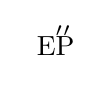
\begin{tikzpicture}[baseline=(root.base)]
\tikzset{every tree node/.style={align=center,anchor=north}}
    \Tree [.\node(root){EP}; {external argument (originator)}
            [.E$'$ E
                [.{Asp\tss{Q}P (inner aspect domain)} theme
                    [.Asp\tss{Q}$'$ Asp\tss{Q} {V (predicate)}
                    ]
                ]
            ]
          ]
\end{tikzpicture}
\end{exe}

While according to the lexicalist approach to argument structure
\citep[cf.][]{Chomsky1970,Reinhart2002}, the roles of event participants are
projected by the predicate which is embedded at the bottom of the functional
structure, in the XS model, the predicate does not contain any syntactic
information such as the thematic grid. The interpretation concerning the theta
roles of event participants and telicity is derived from the functional
structure EP, and the predicate only provides conceptual meaning that modifies
the functional structure. The Asp\tss{Q} head in EP is the counterpart of the
quantity head in DP, responsible for the quantification of the event, and the
valuation of the feature specified on this head is the source of telic
interpretation. Thus, in the XS model, telicity comes from the valuation of the
quantity feature specified on the Asp\tss{Q} head. In languages like \ili{English}, the
valuation of the quantity feature is often achieved via specifier--head
agreement, which can copy the quantity value of a quantity DP in the specifier
position of the Asp\tss{QP} onto the Asp\tss{Q} head, thereby giving rise to the
interpretation of telicity.

We can take the following examples to illustrate the feature valuation of
quantity in EP:

\begin{exe}
    \ex\label{FValQ1} John ate three apples \emph{in five minutes}.
    \ex\label{FValQ2} John ate apples *\emph{in five minutes/for five minutes}.
\end{exe}

Following the XS model, in (\ref{FValQ1}) it is the DP \emph{three apples} in
the specifier of the Asp\tss{QP} that provides the interpretable quantity
feature to value the uninterpretable quantity feature on the Asp\tss{Q} head.
The valuation of the quantity feature then gives rise to the semantic
interpretation of the telicity of the eating event. On the other hand, in
(\ref{FValQ2}), the bare plural \emph{apples} does not bear an interpretable
quantity feature, which means in this sentence, if the Asp\tss{Q} head
projects, the valuation of the quantity feature, and hence telic
interpretation, cannot be achieved.

Just like the DP structure, in EP the functional head\is{functional items} specifying the quantity
feature is optional, which is exactly the case of atelic events. When
Asp\tss{Q} head does not project, which is the case of atelic events, a layer
of F\textsuperscript{\emph{s}}P will appear in the otherwise Asp\tss{QP} position, and the [Spec F\textsuperscript{\emph{s}}P]
position will host a DP that is the theme of the event.\footnote{In
\citeauthor{Borer2005b}'s (\citeyear{Borer2005b}) original model, the
nominal in the [Spec Asp\tss{QP}] takes the role of ``subject of quantity'',
while the nominal in the [Spec F\textsuperscript{\emph{s}}P] position takes the
role of ``default participant''. Abstracting away technical details that do not
concern the discussion in this paper, and for ease of exposition, I will simply
use the term ``theme'' to refer to the DPs in the [Spec AspP] and [Spec
F\textsuperscript{\emph{s}}P] positions.} Since this paper focuses on telicity,
F\textsuperscript{\emph{s}}P will not be discussed.

As mentioned above, in \ili{English}, the quantity feature on the Asp\tss{Q} head is
valued with the indirect strategy: copying the quantity feature of a DP in
[Spec Asp\tss{QP}] via agreement. In theory, it is possible that in some
languages the direct valuation strategy might be available, if there is a
functional item in the lexicon that bears an interpretable quantity feature. In
\textcite{Borer2005b}, it is shown that this situation does exist in some
Slavic languages. In languages like \ili{Czech}, a perfective prefix serves as an
event delimiter, which imposes a telic interpretation on the one hand, and also
restricts the interpretation of bare nominal arguments by providing them with
quantificational force:

\begin{exe}
\ex \ili{Czech} \parencite[62]{filip1997}
    \begin{xlist}
	\ex\label{Filip1} \gll Pil\textsuperscript{\emph{I}} v\'ino.\\
	        {drank-\Sg{}{}} {wine-\Sg{}-\Acc{}} \\
	    \glt \enquote*{He was drinking (the) wine.}
    \ex\label{Filip2} \gll  Vypil\textsuperscript{\emph{P}} v\'ino.\\
            {\Pfv{}-drank-\Sg{}{}} {wine-\Sg{}-\Acc{}} \\
        \glt \enquote*{He drank up (all) the wine.}
\end{xlist}
\end{exe}

In the above example, the prefixed perfective verb gives rise to a telic
interpretation. In     addition, the prefix also forces a definite and quantity
reading on the bare object, as is shown in (\ref{Filip2}). Without the
perfective prefix, no telic reading is attested, and the bare noun does not
need to take a definite reading or quantity reading as shown in (\ref{Filip1}).

\textcite{Borer2005b} takes such data as evidence of the paradigm of direct
range assignment (feature valuation). In particular, a perfective prefix in
Slavic languages is a functional item that bears the interpretable quantity
feature, which is directly merged in the Asp\tss{Q} head to value the
uninterpretable quantity feature ([\emph{u}Quan] for short). In addition, when
a bare nominal theme argument is involved, the perfective prefix copies the
quantity feature to the quantity head in the DP structure, and provides a
strong D feature to value the uninterpretable D feature ([\emph{u}D])
on the D head of the DP, as is the case in (\ref{Filip2}).

\section{Telicity in Yixing Chinese}\label{sec:17.4}

Chinese is not considered in previous studies on the cross-linguistic
variation of telicity, mostly because how telicity is derived exactly in
Chinese is not well understood.\footnote{In the final stage of proofreading
    this paper, I was informed that \textcite{Peng2017} discovered that in
    Chinese dialects like Pingxiang, there are also two distinct particles that
    both correspond to the verbal \emph{le} in Mandarin. Peng also shows that
    one particle is a telic marker, which further supports the analysis made
    here. I would like to emphasise that I am by no means the first to
    correlate telic function with verbal \emph{le} in Mandarin. The crucial
    point made in this paper is how \isi{parameters} of telicity could be derived
with such linguistic phenomena.} The \isi{inner aspect} of Chinese is widely
mentioned in the vast literature on the famous verb particle \emph{le}, which
is often assumed to be related to telicity in one way or another
\citep[cf.][]{smith1997parameter,lin2003aspectual,soh2007over,soh2009speaker,soh2014aspect}.
However, the mechanism of telicity in Chinese is by no means clear, partly
because the verbal \emph{le} does not always give rise to telicity:

\begin{exe}
\ex \ili{Mandarin} \begin{xlist}
	\ex\label{Yixing1} \gll ta wu fenzhong li chi le san ge pingguo. \\
	                        He five minute in eat \textsc{le} three \Clf{} apple \\
	                   \glt \enquote*{He ate three apples in five minutes.}
    \ex\label{Yixing2} \gll  ta (*wu fenzhong li) he le cha le. \\
                            He \hphantom{(*}five minute in drink \textsc{le} tea \textsc{le} \\
                       \glt \enquote*{He has already drunk tea *in five minutes.}
\end{xlist}
\end{exe}

Obviously, without knowing the precise factor determining telicity in Chinese,
it is impossible to bring Chinese into the broad picture of \isi{telicity
    parameter}.  In \textcite{Huxuhui2016}, I used data from \ili{Yixing
    Chinese}\footnote{Yixing Chinese is a variety of Wu dialect,\il{Wu Chinese} spoken
in Yixing county with a population of 1,243,700, a subdivision of Wuxi city in
China’s Jiangsu province.} to show that the verbal \emph{le} in \ili{Mandarin} is not
a homogeneous category, but is the phonological realisation of two homonymous
categories, one being the inner aspectual marker, which is the counterpart of
\emph{lə} in Yixing, and the other is an outer aspectual marker, which
corresponds to \emph{dzə} in Yixing.  In this section, I present the major
properties of \emph{lə} that are closely related to the central topic of this
paper, i.e. the variation of telicity, while leaving other properties aside
(but see \citealt{Huxuhui2016}). To distinguish \emph{lə} from \emph{dzə}, the
properties of \emph{dzə} will also be presented when necessary.

In Yixing, all the achievement and accomplishment predicates with an
incremental theme can occur in a \emph{lə}-marked sentence. In addition, when
\emph{lə} occurs, a telic interpretation arises invariably, as is evidenced by
the compatibility with the Chinese version of the \emph{in x time} phrase. That
is, a \emph{lə}-marked sentence always denotes an atomic event in the sense of
\textcite{Rothstein2004}.

\begin{exe}
\ex Achievement predicate\label{achievement predicate}\\
   \gll {tɔ} {sasə} {fəŋʣoŋ} lidou {mə} \emph{lə} sa bən ʃy. \\
    He thirty minute in lose {lə} three \Clf{} book. \\
    \glt \enquote*{He lost three books in thirty minutes.}
\ex Accomplishment predicate\label{accomplishment predicate}\\
   \gll  {tɔ} {sasə} {fəŋʣoŋ} lidou {ʧε} \emph{lə} sa {ʣə} bɪŋgo. \\
    He thirty minute in eat {lə} three \Clf{} apple. \\
    \glt \enquote*{He ate three apples in thirty minutes.}
\end{exe}

There is evidence that telicity is not the information taken by the predicate
in Yixing. Instead, telicity is directly related to \emph{lə}, as when
\emph{lə} \ is not available, even with a quantised incremental theme and a
homomorphic predicate, still a telic interpretation cannot be attested. For
example, the examples in (\ref{ungram}) will be unacceptable if
\emph{lə} is replaced by another verbal particle or if there is no particle at
all:

\begin{exe}
    \ex\label{ungram} \ili{Yixing Chinese}
    \begin{xlist}
        \ex[*]{
            \gll {tɔ} {sasə} {fəŋʣoŋ} lidou {mə} {$\varnothing$ / ʣə  / go} sa bən ʃy. \\
            he thirty minute in lose {$\varnothing$ / ʣə / go} three \Clf{} book. \\
            \glt intended: \enquote*{He lost three books in thirty
            minutes.}\footnote{$\varnothing$ stands for zero-particle, i.e.,
        the situation when no particle
    occurs.}\textsuperscript{\emph{,}}\footnote{The verbal particle \emph{go},
which is the counterpart of \emph{guo} in \ili{Mandarin}, often indicates that
an event happened before a certain time but does not have an effect on the
topic time (cf.\ \citealt{smith1997parameter,soh2014aspect}).}
        }
        \ex[*]{
            \gll {tɔ} {sasə} {fəŋʣoŋ} lidou {ʧε} {$\varnothing$ / ʣə / go} sa {ʣə} bɪŋ go. \\
            he thirty minute in eat {$\varnothing$ / ʣə / go} three \Clf{} apple. \\
            \glt intended: \enquote*{He ate three apples in thirty minutes.}
        }
    \end{xlist}
\end{exe}

The examples in (\ref{achievement predicate}) and (\ref{accomplishment
predicate}) on the one hand, and (\ref{ungram}) on the other form a minimal
pair, clearly indicating that what plays a crucial role in yielding telic
interpretation is the particle \emph{lə}.

What further augments the above descriptive conclusion is that \emph{lə} may
also force the event with an activity or state predicate to yield a telic
interpretation, although such predicates usually appear in atelic events in
Vendler's classification.

\begin{exe}
\ex \ili{Yixing Chinese} \begin{xlist}
    \ex\label{coerced telic}
    Context: Zhangsan's work is to push the cart with goods from the market to
    the shop, and the following sentence is uttered to express the working load
    Zhangsan has achieved in 30 minutes:\\
    \gll ʣaŋsa {sasə} {fəŋʣoŋ} lidou tae {lə} sa {ʦɔ} ho. \\
    Zhangsan thirty minutes in push {lə} three cart good. \\
    \glt \enquote*{Zhangsan pushed three carts of goods in 30 minutes.}

    \ex \gll ʣaŋsa ʤiŋʣao {jɨ} te lidou {kaeʃiŋ} {lə} sa {ʦi}. \\
    Zhangsan today one day in happy {lə} three time. \\
    \glt \enquote*{Today, Zhangsan became happy three times in one day.}
\end{xlist}
\end{exe}

The events denoted by the above two sentences are telic, evidenced by the
adverbial \emph{in x time}. Although these two sentences involve an activity
predicate and a stative predicate respectively which in most cases appear in
atelic sentences, the telic interpretation is obligatory because of the
presence of \emph{lə}. What is especially noteworthy is that although
\emph{kaeʃiŋ} `happy' is often used as an adjective, it takes a dynamic reading
here denoting a change of state, roughly equivalent to \textit{to become happy} in
\ili{English}. As illustrated below: without \emph{lə}, the above sentences
will be unacceptable:

\begin{exe}
\ex \ili{Yixing Chinese} \begin{xlist}
    \ex[*]
     {\gll ʣaŋsa {sasə} {fəŋʣoŋ} lidou tae {$\varnothing$ / ʣə / go} sa {ʦɔ} ho. \\
    Zhangsan thirty minutes in push {$\varnothing$ / ʣə / go} three cart good. \\
    \glt intended: \enquote*{Zhangsan pushed three carts of goods in 30
    minutes.}\footnote{The context of this sentence is exactly that of
(\ref{coerced telic}).}
    }


    \ex[*]{
    \gll ʣaŋsa ʤiŋʣao {jɨ} te lidou {kaeʃiŋ} {$\varnothing$ / ʣə / go} sa {ʦi}. \\
    Zhangsan today one day in happy {$\varnothing$ / ʣə / go} three time. \\
    \glt \enquote*{Today, Zhangsan became happy three times in one day.}
    }
\end{xlist}
\end{exe}

The previous studies on the verbal \emph{le} in \ili{Mandarin} mainly focus on the
semantic effects relevant to the event, such as whether it denotes a completion
or termination of an event and whether it signals the realisation of a state
that holds at the \isi{topic} time. The possible relationship between verbal
\emph{le} and the nominal theme is never considered. With Yixing data, the
quantificational effect of \emph{lə} over the nominal theme of the event is
brought to our attention. In Yixing, \emph{lə} occurs in a sentence where the
nominal theme has a quantity reading. Whenever a non-quantity reading is
imposed on the nominal theme, the sentence will be unacceptable. As I will show
shortly, bare nouns can be the theme of the verbs marked with \emph{lə}; when
this occurs, the bare noun will not have the mass reading or bare plural
reading,\footnote{Like \ili{Mandarin}, Yixing does not have a plural marker in
general, so nominals with mass and bare plural readings both have the form of
bare nominals.} but will be forced to take a specific and quantity reading.
Therefore, the requirement of the quantity theme can be met in two situations.
Firstly, \emph{lə} can co-occur with a nominal that involves an overt numeral,
clearly indicating quantity:

\begin{exe}
    \ex \ili{Yixing Chinese}\\
   \gll {tɔ} {ʧε} \emph{lə} sa {ʣə} bɪŋgo. \\
    He eat {{lə}} three \Clf{} apple. \\
    \glt \enquote*{He ate three apples.}
\end{exe}

If a bare nominal occurs as the theme with a mass or bare plural
interpretation, the sentence will be ungrammatical:

\begin{exe}
\ex \ili{Yixing Chinese} \begin{xlist}
    \ex[*]{
    \gll {tɔ} {ʧε} \emph{lə} {ʤu} \emph{lɨ}. \\
    He eat lə alcohol lɨ. \\
    \glt intended: \enquote*{He has had alcohol.}
    }

    \ex[*]{
    \gll {tɔ} {ʧε} \emph{lə} bɪŋgo \emph{lɨ}. \\
    He eat lə apple lɨ. \\
    \glt intended: \enquote*{He has had apples.}
    }
\end{xlist}
\end{exe}

A bare nominal theme, if it is to be compatible with \emph{lə}, must have a quantity
and definite specific reading. This quantity/definite reading is possible when
the bare nominal is fronted to a \isi{topic} construction. Three positions are
possible if the object is taken as the \isi{topic} in Yixing (and in Mandarin):
clause initial position, the position in between the subject and the verb
(SOV), and the complement position of \emph{ba},\footnote{In \ili{Mandarin}, \emph{ba}
occurs after the subject and takes the object in its complement position,
where the object is often interpreted as the \isi{topic}. Its counterpart in Yixing is
\emph{nɔ}, which works exactly like \emph{ba}. For a comprehensive description
and analysis of the \emph{ba}-construction, see
\textcite[153--196]{HuangEtal2009}.} which is \emph{nɔ} in Yixing. These three
positions all can hold the bare nominal object when it co-occurs with
\emph{lə}.\footnote{This description ignores possible underlying structural
    differences, which aren’t crucial here.} In the following examples, the
    bare noun \emph{ʤu} `alcohol' has a quantity and specific interpretation:
    for such examples to be grammatical, it has to mean a certain quantity of
    alcohol, as well as the presupposition that this quantity of alcohol is
    known to both the hearer and the speaker.\footnote{For an account of
    fronting\is{fronting!of arguments} the object in these examples, see
\textcite{Huxuhui2016}.}

\begin{exe}
    \ex \ili{Yixing Chinese}\\
     \gll {ʤu} ŋo {jiʤiŋ} {ʧε} \emph{lə} lɨ. \\
    alcohol I already eat lə lɨ. \\
    \glt \enquote*{I have drunk the alcohol (i.e. the certain amount of alcohol has been drunk up by me).}

    \ex \ili{Yixing Chinese}\\
  \gll ŋo ʤu {jiʤiŋ} {ʧε} \emph{lə} lɨ. \\
    I alcohol already eat lə lɨ. \\
    \glt \enquote*{I have drunk the alcohol (i.e. the certain amount of alcohol has been drunk up by me).}

\ex \ili{Yixing Chinese}\\
   \gll ŋo {jiʤiŋ} {nɔ} ʤu {ʧε} \emph{lə} lɨ. \\
    I already {nɔ} alcohol eat lə lɨ. \\
    \glt \enquote*{I have drunk the alcohol (i.e. the certain amount of alcohol has been drunk up by me).}
\end{exe}

We can thus draw a descriptive conclusion: a quantity theme is an obligatory
requirement of \emph{lə}. This requirement is met when a nominal phrase already
takes a quantity feature provided by the numeral; if a numeral is not available
as is in the case of bare nominals, \emph{lə} seems to ``offer'' a quantity
interpretation. In \textcite{Huxuhui2016}, following \textcite{Borer2005b}, it
is argued that this is made possible because the quantity feature of the telic
item \emph{lə} is copied onto the nominal in the [Spec Asp\tss{Q}] position,
thus presenting a symmetry with the situation in \ili{English}: In \ili{English}, without a
functional telic item, the quantity feature of a DP in [Spec Asp\tss{Q}] has to
be copied on the Asp\tss{Q} head, while in Chinese, with the feature provided
by the telic item, the quantity feature on Asp\tss{Q} head is copied onto the
nominal phrase in [Spec Asp\tss{Q}].

\section{Exploring the telicity parameter}\label{sec:17.5}
\subsection{An initial account}

So far, with both Chinese, \ili{English} and \ili{Slavic} data, it seems that
telic variation can be neatly accounted for with Borer's XS model. All the
cross-linguistic issues can be reduced to a single factor: whether there is a
functional item specifying quantity feature in the lexicon\footnote{I am
    assuming the proposal initiated in \isi{Distributed Morphology}
    \citep[cf.][]{HalleMarantz1993,marantz2007phases} that a lexicon of a
    language has both \isi{functional items} and lexical items, with the former
    specifying features to be engaged in syntactic computation, and the latter
mainly takes conceptual meaning.}, which can be directly merged in the
Asp\tss{Q} head to value the uninterpretable quantity feature on this
functional head\is{functional items} (`Asp quantity feature', to be
distinguished from the quantity feature of DP).

The parameter of telicity can therefore be summarised below:\is{telicity
parameter}

\begin{exe}\ex Telicity parameter (first version)\smallskip\\
\begin{tikzpicture}[thick,scale=0.9, every node/.style={scale=0.94}]
\tikzset{every tree node/.style={align=center,anchor=north}}
    \Tree [.{Does the lexicon contain a functional item bearing an Asp quantity feature?} {Yes (direct telic languages)\\Chinese (Mandarin, Yixing and other dialects)\\Slavic languages...} {No (indirect telic languages)\\English and other\\\ili{Germanic} languages...} ]
\end{tikzpicture}
\end{exe}

In the above division, I use the term direct telicity language
(\glsunset{DT}\gls{DT} language for short) to refer to languages that contain a
functional item to directly value the feature on the inner aspectual \is{inner aspect}head,
while indirect telicity language (\glsunset{IT}\gls{IT} language for short)
refers to those that have to adopt an indirect mechanism such as spec-head
agreement to value this feature. The above single parametric factor results in
the cluster of differences in~\Cref{table:1}.

\begin{table}
\caption{Properties of DT and IT languages (first version)}\label{table:1}
\begin{tabularx}{1\textwidth}{lQQQ}
\lsptoprule
{} & Does telicity rely on quantity objects? & Does telicity provide quantity reading to bare nominals? & Does quantity object impose telicity? \\
\midrule
DT languages\textsuperscript{\itshape a} & no  & yes & no\\
IT languages\textsuperscript{\itshape b} & yes & no & yes\\
\lspbottomrule
\end{tabularx}
\footnotetext[1]{(Chinese, \ili{Slavic} Languages)}
\footnotetext[2]{(English and other \ili{Germanic} languages)}
\end{table}

\Cref{table:1} shows that a single \isi{telicity parameter} based on the
existence of a functional item bearing the quantity feature is the underlying
reason for a range of cross-linguistic variations. I have already shown at
different points in this paper that for Chinese and \ili{Slavic} languages, telic
reading does not rely on the quantity object. What is crucial is the presence
of the inner aspectual \is{inner aspect}functional item. On the other hand, for languages like
English which lacks such a functional item, the indirect feature valuation of
the quantity feature on the inner aspectual \is{inner aspect}head is taken, which relies on the
copying of the quantity feature of the DP in the [Spec Asp\tss{QP}] position.
This explains why languages like \ili{English} have to rely on the quantity nominal
object to derive telic reading. The same parametric difference also directly
explains why quantification over bare nominals only occur in DT languages: the
functional item bearing a quantity feature can scope over the bare nominal in
the [Spec Asp\tss{QP}] position, while in IT languages like \ili{English}, without
such a functional item, naturally this type of quantification is impossible.

So far, the parametric account of telicity is completely based on Borer's
(\citeyear{Borer2005b}) XS model, and this paper provides data from Yixing to
further support this account: Borer's account predicts that it is possible that
a quantity functional item might exist in other languages other than
Slavic\il{Slavic} languages, and Yixing\il{Yixing Chinese} data confirm this
prediction.

\subsection{Telicity parameter: A further specification}\label{sub:17.5.2}

\textcite{huang2015syntactic} points out that Chinese verbs seem to be
inherently atelic, which can be illustrated by the following
examples,\footnote{Since the verbal \emph{le} in \ili{Mandarin} can be either
    an outer or inner (telic) marker, to avoid confusion, we use Yixing in this
paper to illustrate relevant points in Chinese.} an observation also noticed in
\cite{tai1984} and \textcite{smith1997parameter}.

\begin{exe}
    \ex\label{inherently atelic} \ili{Yixing Chinese}\\
\gll ʣaŋsa {sasə} {fəŋʣoŋ} lidou {ʃε} {lə} sa {foŋ} {ʃiŋ}, dazi {jɨ} {foŋ} a {mə} wəʣəŋ. \\
    Zhangsan thirty minute in write {lə} three \Clf{} letter, but one \Clf{} even not complete. \\
    \glt \enquote*{Zhangsan wrote three letters in thirty minutes, but none of the letters was completed.}
\end{exe}

Even with the marker \emph{lə} in Yixing,\il{Yixing Chinese} still the action
does not seem to have an endpoint because the three letters are not finished.
In order to guarantee the information of completeness, a ``completeness
particle'' has to be attached to the verb. Note that there are different
completeness particles in Chinese, which match different verbs. This fact
carries over to Yixing. Below I use a Yixing example for the sake of
consistency, wherein \emph{wə} (counterpart of \emph{wan} in Mandarin) is a
completeness particle.

\begin{exe}
    \ex\label{*completeness} \ili{Yixing Chinese}\\
    \gll ʣaŋsa {sasə} {fəŋʣoŋ} lidou {ʃε-\emph{wə}} {lə} sa {foŋ} {ʃiŋ},
    \llap{*}dazi {jɨ} {foŋ} a {mə} wəʣəŋ. \\
    Zhangsan thirty minute in write-finish {lə} three \Clf{} letter, but one \Clf{} even not complete. \\
    \glt \enquote*{Zhangsan finished writing three letters in thirty minutes,
    but none of the letters was completed.}\footnotemark
\end{exe}
\footnotetext{Note that the symbol ``*'' in (\ref{*completeness}) does not mean
the clause itself is ungrammatical, but only shows that the information
expressed by the clause contradicts that of the preceding clause. This also
applies in the following examples of this section.}

This appears to contradict the assumption that \emph{lə} is a telic marker that
imposes telic interpretation. Huang's (\citeyear{huang2015syntactic})
explanation is that Chinese verbs are inherently atelic and thus a completeness
particle is required to denote telic events. However, this account is
problematic considering the fact that the completeness particle on the one hand
cannot guarantee the derivation of telicity, and on the other hand telicity can
arise even without such particles. As I have already shown in this paper,
without \emph{lə}, a telic sentence will not be acceptable, and the data also
show that many \emph{lə}-marked telic sentences do not need completeness
particles. So here is a puzzling issue: on the one hand, \emph{lə} does seem to
take the responsibility of marking telicity, but on the other hand, without a
completeness particle, the event, at least in the traditional assumption, does
not always express an endpoint.

To address the above puzzle, the clarification of ``endpoint'' is crucial.
Concerning the data in (\ref{*completeness}), ``endpoint'' is often understood as
the point when the whole event is measured out by the theme argument: if the
matrix verb is a consumption verb, the endpoint is understood as the point when
the final bit of the food is consumed. If we think further, we will realise
that this type of endpoint does not equate to the endpoint in defining
telicity.  The interpretation of a telic event comes from the linguistic
expression of an endpoint of an event. Here, what is at stake is that the
linguistic derivation explicitly provides the information that the event ends
at a point, regardless of whether this is the point when the event is measured
up by the object. With this in mind, I posit the following hypothesis:

\begin{exe}
\ex\label{le hypothesis} \emph{lə} in Yixing (and the inner aspectual \is{inner aspect}\emph{le} in Mandarin), as a pure telic functional item, provides the abstract meaning (semantic feature) that the event ended at a certain point.
\end{exe}

Note that the above hypothesis about the semantic contribution of \emph{lə} is a natural consequence of the assumption that \emph{lə} is a pure telic marker. Since, as I have pointed above, telicity is characterised with the endpoint of an event, a telic marker should be responsible for introducing this semantic characteristic. This means that as long as \emph{lə} is involved in the sentence, an endpoint is expressed linguistically, and this endpoint does not have to be the point when the event is measured up by the object. For the convenience of exposition, I term the latter type of point as measuring up point, to be distinguished from endpoint.

For \emph{lə}-marked sentences with canonical accomplishment verbs, the default
interpretation is that the event reaches an endpoint when the event is measured
up by the object. This is so because to the language user, the measuring up
point is the most accessible endpoint of such events. However, as long as there
is supporting contextual information, such a default interpretation can be
cancelled. This is exactly the situation of the example in (\ref{inherently
atelic}). The second clause indicates that the event was not measured up by
\enquote{the three letters}. Since the telic marker \emph{lə} provides the explicit
information that the event of writing three letters ended at a certain point,
and since the second clause cancelled the identification of the endpoint with
the measuring up point, we are forced to take another interpretation that in
this event, the agent had the plan to write three letters, but he ended this
writing event without completing any of the three letters. This event is still
telic, because it is explicitly expressed that the event arrived at an
endpoint, while how much the agent had written for each letter was not
specified. The \emph{in x time} diagnostic in (\ref{inherently atelic}) also
shows that this sentence, although lacking a measuring up point, is telic.


Now we have to address this question: why is it so that for the telic accomplishment events in \ili{English}, the endpoint is always identified with the measuring up point?

\begin{exe}
\ex John ate three apples in 5 minutes, *but he did not eat up any of the apples.
\ex John wrote three letters in 3 hours, *but none of the letters was completed.
\end{exe}

This question can be addressed by the mechanism of feature valuation for the derivation of telicity. Note that in \ili{English}, no functional telic item is available in the lexicon, and telicity arises when the quantity feature of the object DP is copied onto the Asp\tss{Q} head. A semantic consequence of this syntactic operation is that the endpoint expressed by the sentence must be identified with the measuring up point: after all, the interpretable quantity feature assigned to the inner Asp\tss{Q} head is exactly the quantity feature of the object DP, and the identification of the endpoint and the measuring up point is the reflection of this syntactic operation. This identification is imposed by syntactic operation, and therefore is not cancellable, but part of the semantic meaning that contributes to the truth value of the proposition.


Following the analysis developed so far, it can be predicted that if a language
has a functional item that can directly value the feature on the inner
Asp\tss{Q} head, the situation of the Chinese example in (\ref{*completeness})
should also occur in this language. But the \ili{Slavic} data seem to invalidate this
prediction: I have argued, following \textcite{Borer2005b}, that the perfective
prefixes in \ili{Slavic} languages are \isi{functional items} that provide the
interpretable quantity feature to the inner Asp\tss{Q} head. This implies that
such prefixes are in nature equivalent to \emph{lə} in Yixing. Considering the
hypothesis in (\ref{le hypothesis}), the identification of the event endpoint
with the measuring up point in \ili{Slavic} languages should also be a piece of
cancellable default information. This prediction does not hold, though, as
shown by the following \ili{Czech} examples:\footnote{I thank Eva Roubalov\'a for
providing these two examples and Nong Xi for providing further clarification
with the data.}

\begin{exe}
\ex \ili{Czech} \begin{xlist}
    \ex \gll Dneska jsem \textit{na}psal p\v{e}t dopis\r{u}, \llap{*}ale ani jeden z nich jsem ne-\textit{do}psal. \\
        Today I {wrote-\Pfv{}-\Sg{}{}} {five-\Acc{}} {letter-\Pl{}-\Poss{}} but even one of them I {not-finished writing-\Pfv{}-\Sg{}} \\
        \glt \enquote*{Today I wrote five letters, but I finished none of them.}
    \ex \gll B\v{e}hem p\v{e}t m\v{e}s\'ic\r{u} jsem \textit{pře}četl dv\v{e}
    knihy, \llap{*}ani jednu z nich jsem ne-\textit{do}četl.\\
        Within {five-\Poss{}} {month-\Pl{}-\Poss{}} I {read-\Pfv{}-\Sg{}{}} {two-\Acc{}} {book-\Pl{}-\Acc{}} even one of them I {not-finished reading-\Pfv{}-\Sg{}} \\
        \glt \enquote*{In five months I have read two books, but I did not finish reading either of them.}
    \end{xlist}
\end{exe}

I postulate the following hypothesis on the nature of perfective prefixes in \ili{Slavic} languages:

\begin{exe}
\ex\label{perf hypo} The perfective prefixes in \ili{Slavic} languages like \ili{Russian} and \ili{Czech} have double functions:
    \begin{description}
        \item[Function A (Semantic function):] A \ili{Slavic}
            perfective prefix functions as a lexical particle that enriches the
            lexical information, i.e. conceptual meaning, of the verb; more
            specifically, it provides the information entailing the
            identification of the endpoint of an event with the measuring up
            point.
        \item[Function B (Syntactic function):] A \ili{Slavic} perfective prefix can work as a functional item that values the quantity feature on the inner Asp\tss{Q} head.
    \end{description}
    Function A is invariable, while function B is optional.
\end{exe}

Explanation of the above hypothesis is in order. Function A is largely in line with the proposal made in \textcite{filip2005telicparameter} and \textcite{filiprothstein2005} that \ili{Slavic} perfective prefixes are lexical operators applied to verbal predicates, an assumption also in line with \textcite{partee1995quantification}. This assumption equates prefixes in \ili{Slavic} with Chinese completeness particles, both contributing concrete lexical information to the predicate. In fact, when \ili{Slavic} prefixes and Chinese completeness particles are viewed together, we can see their surface similarities: both \ili{Slavic} prefixes and Chinese completeness particles have different forms corresponding to different predicates; both contribute the lexical information of the entailment that the endpoint of the event is the measuring event. Note that if we take the assumption that telicity is the result of feature valuation, then such lexical items, either the \ili{Slavic} prefixes or Chinese completeness particles, cannot give rise to telicity because they are not functional (inflectional) items. This is the case in Chinese: I have shown that Chinese completeness particles alone cannot yield telicity. But \ili{Slavic} prefixes do have the function of yielding telicity. This is due to function B: in addition to the lexical information, \ili{Slavic} prefixes also take an interpretable feature, i.e. the quantity feature. This explains why on the one hand telicity is yielded by the perfective prefix in \ili{Slavic}, and on the other hand, the entailment of the identification of the endpoint with the measuring point is also attested.

It then follows that a \ili{Slavic} perfective prefix takes the functions
undertaken by completeness particles and \emph{lə} respectively in Chinese.
Therefore, a prediction we can make is that to denote the semantic information
yielded by the \ili{Slavic} perfective prefix, i.e. both telicity and the
endpoint identification with measuring up point, in Yixing both a completeness
particle and \emph{lə} are required. This is exactly the case of the example in
(\ref{*completeness}).

The hypothesis in (\ref{perf hypo}) also claims that function B, i.e. the
function of serving as a functional item, is optional. The consequence is that
we can expect that more than one prefix can be stacked on a single verb in
\ili{Slavic}, with only one prefix undertaking function A. This is a fact
pointed out by \textcite{filiprothstein2005}, who take this fact to argue
against Borer's (\citeyear{Borer2005b}) hypothesis of taking perfective
prefixes as telic \isi{functional items}: if a perfective prefix is a
functional item, it should not be expected to co-occur with another perfective
prefix attached to the same verb. Now with the hypothesis in (\ref{perf hypo}),
it is clear that when the stack of two perfective prefixes occurs, one of them
is only a lexical particle,\footnote{This assumption implies that if a
perfective prefix only takes function A, it is not a functional item but a
lexical one, and hence should be merged in a position different from that of
both function A and B. In this paper, we do not go further to explain the
syntactic position of the lexical item. We concur with
\textcite{basilico2008syntactic} that it is a Root merged to the Root of the
verb.} while the other serves as a telic functional item.

The above analysis shows that the DT languages in \Cref{table:1} do not constitute a
homogeneous type, but can be further divided depending on the properties of the
telic functional item. The parameter hierarchy\is{parameter hierarchies} of
telicity can thus be enriched, presenting a more fine-grained picture
below:

\begin{exe}
\ex Telicity parameter (revised version)\smallskip\\
\begin{tikzpicture}[thick,scale=0.9, every node/.style={scale=0.94}]
\tikzset{level distance=70pt}
\tikzset{every tree node/.style={align=center,anchor=north}}
    \Tree [.{Does the lexicon contain a functional item\\ bearing an Asp quantity feature?}
        [.{Yes (direct telic languages)\\
                Does the functional item provide\\
                lexical information entailing\\
                the measuring up point?}
            {Yes \\Slavic languages}
            {No \\ Chinese (Mandarin, Yixing,\\and other dialects)} ]
        {No (indirect telic languages)\\English and other \ili{Germanic}\\languages...} ]

\end{tikzpicture}
\end{exe}

It should be noted that only a small number of languages are mentioned in the
above hierarchy. I assume that most, if not all, languages can fit into this
hierarchy\is{parameter hierarchies} depending upon the properties of their
lexicons regarding telic \isi{functional items}. The above hierarchy of
parameters follows the spirit of parametric variation articulated in
\textcite{RobHol2010} as well as the ReCoS project \citep{robertsonline}, which
resolves the tension between micro and macro \isi{parameters}. In this sense, this
research contributes to the research of ReCoS by adding a new hierarchy of
parameters\is{parameter hierarchies} to the broad picture of comparative syntax
detailed by the various studies conducted in this project.  Another potential
contribution of this analysis is that the
\glsunset{BCC}\gls{BCC}\is{Borer--Chomsky conjecture} style parametric variation can be
reduced not only to the formal features in the lexicon, but also to whether a
functional item also bears some lexical information. This assumption is not
confined to the analysis of telic \isi{parameters}, but also carries over to a wide
range of syntactic issues in Chinese \citep[cf.][Ch.\
4]{huang2015syntactic,hu2018encoding}.


The classification of the linguistic properties listed in \Cref{table:1}, accordingly,
needs to be expanded by adding the further classification in~\Cref{table:2}.

\begin{table}
{\small
\caption{Further classification of DT languages\label{table:2}}
\begin{tabularx}{\textwidth}{lQQQ}
\lsptoprule
& Telic functional item(s) available in the lexicon? & Telic functional item contributing lexical information? & Telic sentence entailing the identification of endpoint with measuring up point? \\
\midrule
Chinese & yes & no & no \\
Slavic lgs. & yes & yes & yes\\
\lspbottomrule
\end{tabularx}}
\end{table}

\section{Conclusion}\label{sec:17.6}

This paper takes a basic theme of \textcite{Borer2005b} that telicity is not
part of lexical information, but the result of syntactic derivation via the
standard feature valuation mechanism in Minimalism
\citep{Chomsky2000,Chomsky2001}. I argue, relying on the description and
analysis of \ili{Yixing Chinese} in \textcite{Huxuhui2016}, that like
\ili{Slavic}
languages, Chinese also has a functional telic item that values the quantity
feature on the inner aspectual \is{inner aspect}head.  Further, it is proposed
that Chinese differs from \ili{Slavic} languages in that the telic functional item in
the latter also contributes lexical information that entails the identification
of event endpoint with the measuring up point. A tiny difference in these
properties will lead to a cluster of variation among languages, which is in
line with the broad implication of the hierarchy of parameters\is{parameter
hierarchies} articulated in \textcite{RobHol2010} as well as the ReCoS project
summarised in \textcite{robertsonline}. With a close scrutiny of the
completeness particles and verbal \emph{lə} in \ili{Yixing Chinese} and the
perfective prefix in \ili{Slavic} languages, this paper also explicates how the
lexical information and syntactic features specified on these items (particles
or prefixes) interact in deriving the surface semantic interpretation. This
line of explanation thus provides further issues and perhaps new perspectives
on the recent assumptions about semi-functional items in
\textcite{huang2015syntactic} and the multi-functionality hypothesis of
particles in \textcite{Biberauer2017,Biberauer2017c}.


\pagebreak
\printchapterglossary{}

\section*{Acknowledgements}\largerpage

This research has benefited from discussions with Theresa Biberauer, Alison
Biggs, C.-T. James Huang, Joe Perry, and Ian Roberts. Parts of this paper were
presented at the 24th annual conference of the International Association of Chinese
Linguistics (IACL 24) at Beijing Language and Culture University (BLCU), July
2016, and at the Australian Linguistic Society conference, Monash University,
Melbourne, December 2016. Yingyi Li, Yuchen Liu and Zhouyi Sun provided
important help with typesetting and proofreading the manuscript. The
author is responsible for all potential errors. This research is funded by
the National Social Science Fund of China, No.\ 18BYY044,
\enquote{Neo-constructional approach to syntax: With special reference to
Yixing dialect}.

{\sloppy\printbibliography[heading=subbibliography,notkeyword=this]}

\end{document}
